\section{Problem definitions}
\label{sec:problem} % Arash

In this section, we present a summary of the state of the art of automotive risk assessment methods and discuss their limitation and the impact of these limits. 

Safety means avoiding risk. The risk associated with driving comes from multiple sources. It could be a traffic situation in which a sequence of possibly uncorrelated actions leads to an accident. The risk could also be due to technical failure originating from a system fault. Traffic safety aims at avoiding the former, while the later falls within the scope of functional safety. 

Risk, however, cannot be entirely avoided. The goal of functional safety is to avoid \emph{unreasonable} risk\footnote{Unreasonable risk is judged according to the society's acceptance of the level of risk.} that is due to some malfunctioning. There is always a certain amount of residual risk remaining after taking risk avoidance/mitigation measures. Understanding the risk and measuring it is crucial for directing the effort on avoiding or mitigating the impacts. Moreover, formulating an opinion about when using a system is ``safe enough'' depends on the ability to measure the risk. 

The ISO 26262:2018 [1] captures the State of the art in automotive functional safety. It defines the safety lifecycle and the related safety activities such as Hazard Identification and Risk Assessment. The new international standard ISO/PAS 21448 [2] on Safety of the Intended Functionality aims at the safety of highly automated systems. Other methodologies such as STPA [3] give guidelines on safety engineering based on systems theory. 
From the mentioned sources, the only one that offers a framework for measuring risk is ISO 26262. It defines risk as:
\begin{definition}
	``combination of the probability of occurrence of harm and the severity of that harm.'' 
\end{definition}

This standard gives guidelines to assess risk based on vehicle level hazardous events. A hazardous event is the combination of a vehicle level hazard with operational situation or scenario. It requires analyzing each hazardous event risk individually based on three parameters of Severity, Probability of exposure, and Comparability. The combination of these parameters contributes to constructing the Automotive Safety Integrity Level (ASIL). In this framework, each parameter is quantified in three or four levels that construct the ASIL ranking A, B, C, D, and QM. Where ASIL A represents the least critical level and in ascending order, ASIL D the most critical level. Quality Management (QM) means that the identified hazard is not critical enough for the safety processes, and the quality management system of the manufacturer should suffice for reducing the risk. We depict the ASIL ranking graph in \cref{Fig:ASILGraph}. 

\begin{figure}
	\centering
	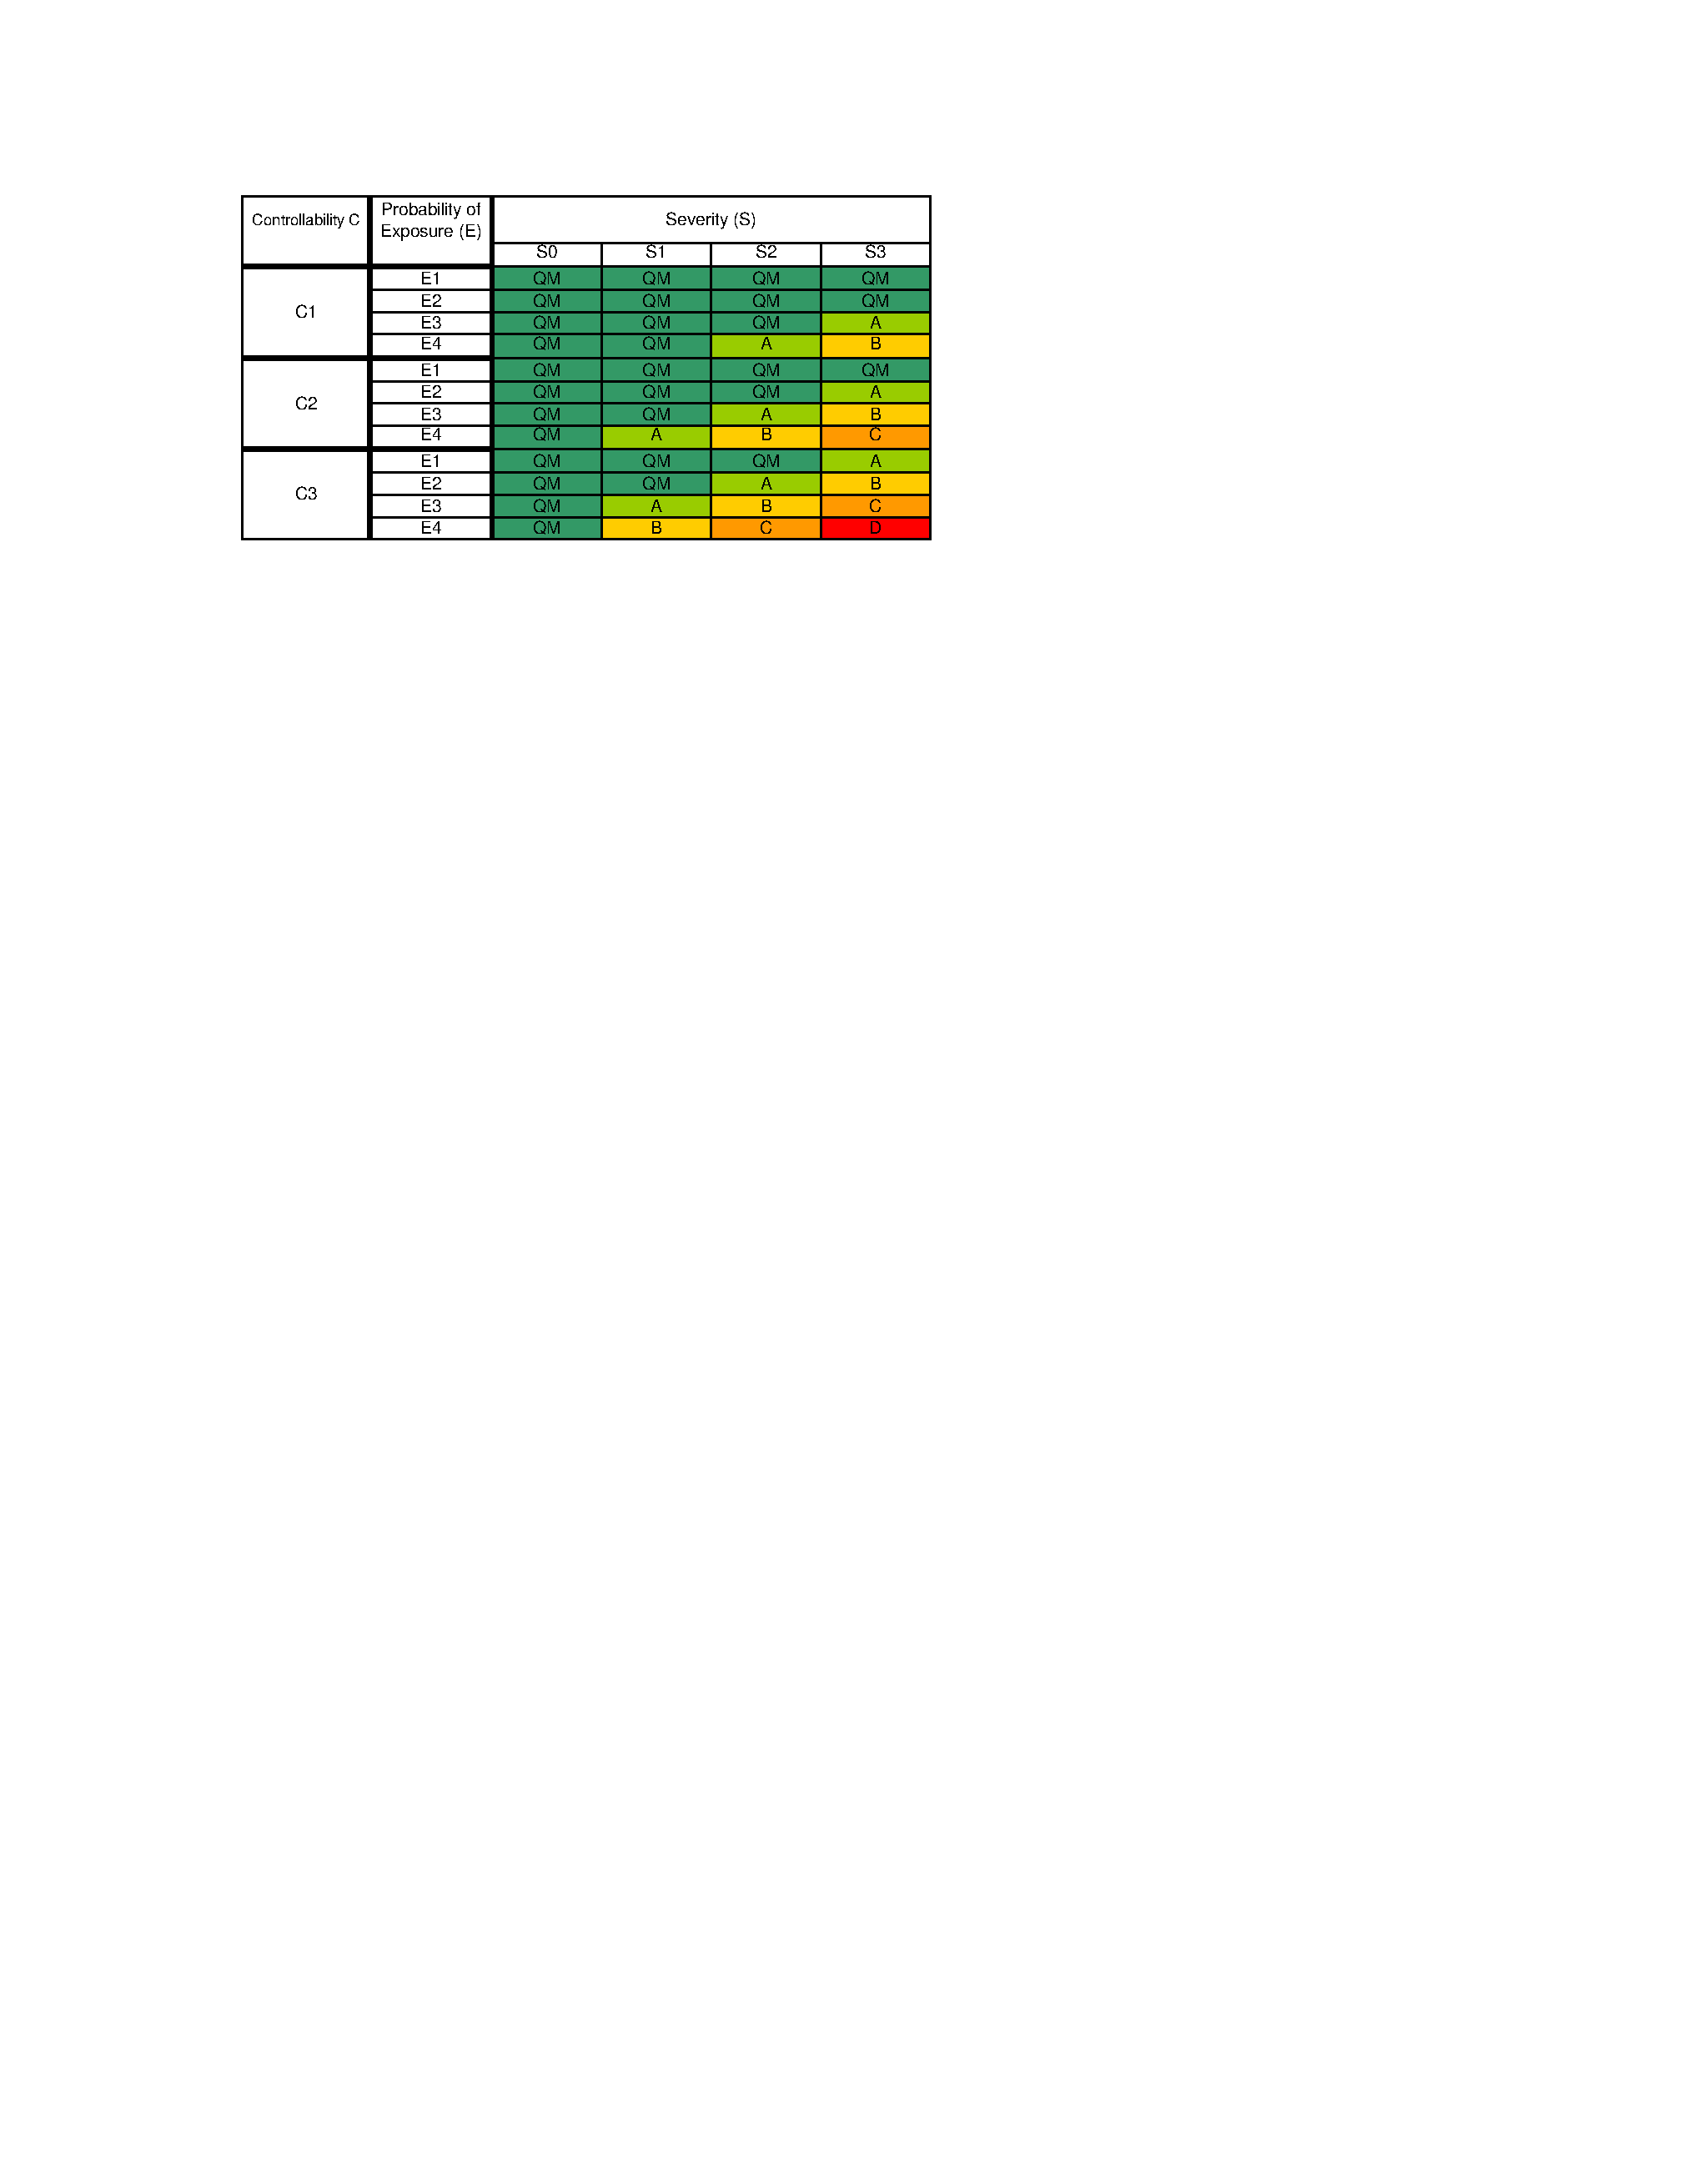
\includegraphics[width=0.9\linewidth]{./figures/ASIL}
	\caption{ASIL Risk Assessment Graph.}
	\label{Fig:ASILGraph}
\end{figure}

The ASIL methodology for risk assessment relies on the experts’ judgments of the three risk parameters. The ISO 26262 provides some general guidelines for assessing these parameters. However, the assessment is for the most part subjective and dependent on the experts who carry it out. 

The alternative methodology proposed in STPA has the means for providing a quantitative risk assessment as it provides the means for connecting the hazard identification to a control system and its characteristics. However, this method skips the risk assessment entirely and does not offer any solutions. 

We argue that as the automotive systems move towards higher automation levels, we require more formal methods for risk assessment. By quantifying risk assessment, we reduce the risk of subjective errors in judgment. Risk quantification is a step towards run-time risk assessment for the autonomous systems.  


